\documentclass[../main.tex]{subfiles}

\begin{document}

\chapter{Introduction}
With the rise of the modern internet more and more systems become digital.
This transformation goes hand in hand with the collection of unprecedented amounts of data leading to the age of big data.
On the on hand, this enables great possibilities for data-driven technologies to improve living conditions in our complex modern world.
On the other hand, it also introduces the risks such as surveillance and the abuse of power.
This observation leads to the fundamental question of the ongoing digital transformation: How can data be used to drive innovation while protecting privacy?~\cite{Boes2022, Schallmo2016}

The novel concept of \emph{Inverse Transparency}~\cite{Boes2022} is concerned with this question.
It aims to provide true data sovereignty for individuals while allowing the sensible usage of data to support digital innovation.
This is achieved by tracking each access to sensitive data.
Whenever a data consumer requests, aggregates, or analyses data of individuals a log is created.
Data owners gain transparent insights into the usage of their data through those logs:
Who accessed which of my data and why?
Moreover, data owners can define policies that restrict access to their data for data consumers.
Only explicitly allowed data accesses are valid and succeed.
This enables true data sovereignty because any harmful data usage can be discovered and may therefore be legally prosecuted.

\citeauthor{Zieglmeier2021}~\cite{Zieglmeier2021} proposed a technical framework supporting this concept.
In their work, they implemented a proof-of-concept toolchain.
\cref{fig:toolchain} is taken from their publication and shows the major components of the approach.
It consists of two actors: The data owner and the data consumer.
The latter aims to access some sensitive data of the former.
Each data access is tracked by a monitor component (\emph{Monitor}) which sends the log to a dedicated server (\emph{Safekeeper}).
A front-end application (\emph{Display}) makes all data accesses transparent to a user by visualizing the captured logs.
It also allows data owners to define policies restricting access to their data.

\begin{figure}[ht]
    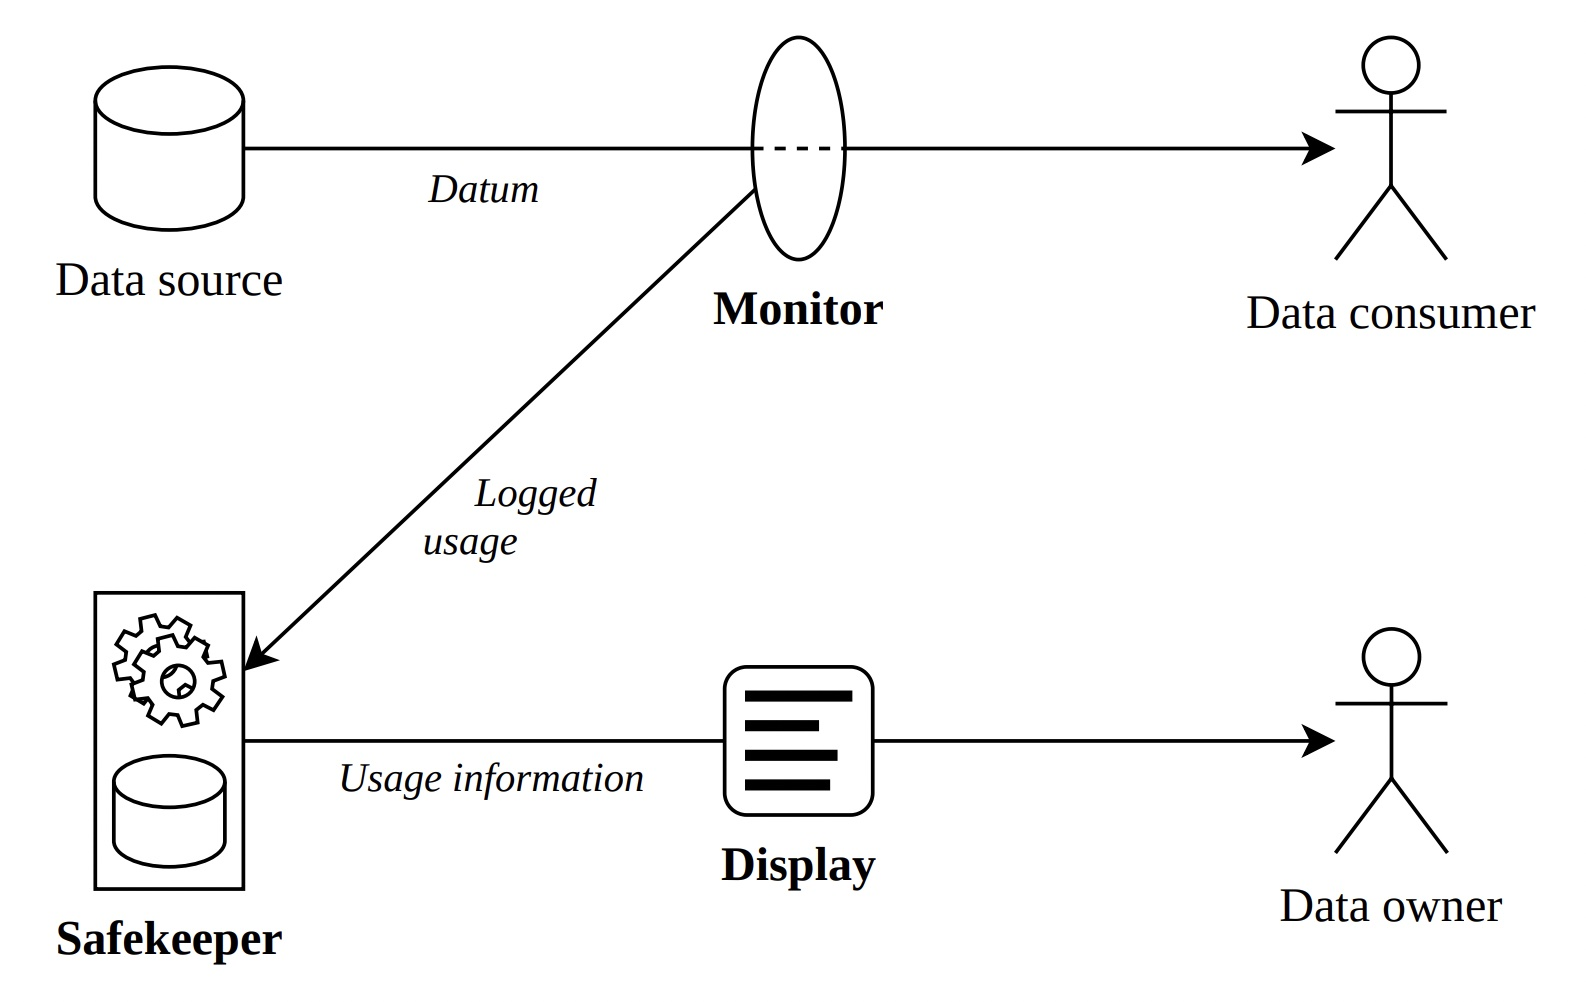
\includegraphics[scale=0.15]{../img/01/toolchain.jpg}
    \centering
    \caption[Existing toolchain]{The structure of the technical framework as proposed by \citeauthor{Zieglmeier2021}~\cite{Zieglmeier2021}.}
    \label{fig:toolchain}
\end{figure}

\subsubsection{Problem statement}

It is crucial to the concept of \emph{Inverse Transparency} that all data accesses are tracked.
The illegal processing of data does not become legal, however, simply because the data owner is informed transparently about the processing~\cite{Boes2022}.
The harmful usage must therefore be legally prosecuted.
This motivates the idea that tracked data accesses can be shared in the system.
If a data owner assumes that a given data access does not adhere to the data privacy regulations the log can be forwarded to the legal department.
Consequently, a data owner should be able to specify certain users in the system who additionally can access the respective log.
A revoking mechanism could further provide the possibility to withdraw access to a log (e.g. because the legal department has finished processing or because the log was shared accidentally).
This ensures that the data owner has full control over the recorded logs.

An important concern is the confidentiality of the collected logs.
The communication between the servers in the toolchain is usually secured and encrypted via TLS~\cite{Rescorla2000}.
The processing servers (e.g. the \emph{Safekeeper}), however, have full access to the logged data.
This introduces several risks.
First, the stored logs contain metadata about the tracked data access (e.g. a justification or the type of data that was accessed).
Recent research shows that the analysis of metadata potentially undermines privacy~\cite{Greschbach2012,Mayer2016}.
Since the log itself might contain sensitive information it should be protected from unintended usage.
Second, \citeauthor{Zieglmeier2021}~\cite{Zieglmeier2021} argue that their conceptual framework is instantiated by companies that have full access to the servers over which the toolchain is deployed.
This generic approach enables great flexibility.
Given the fact that most companies rely on cloud computing~\cite{Weber2021}, however, this introduces the problem that the data might be stored on untrusted third-party servers.
To avoid unintended access to the stored logs the data passing those servers should be encrypted.

\subsubsection{Contribution}

This thesis contributes to the toolchain by designing and implementing an end-to-end encrypted protocol that allows data owners to share and revoke access to their logs.
Specifically, the thesis 
(1)~designs a protocol based on a survey of multi-party encryption techniques
(2)~implements the designed protocol and publishes it for the programming languages Typescript, Go, and Python
(3)~integrates the implemented protocol into the existing toolchain, and 
(4)~evaluates the implemented protocol in terms of functionality, security and performance.

\subsubsection{Outline}
\todo{Outline}

\end{document}